

\section{Finite Size Methods}

In the Ising model spins tend to form clusters, which adds a spatial correlation to the time correlation. Quantities already introduced in \citet{comp_phys} and \eqref{eq:corr_len} (the \emph{correlation} and the \emph{correlation length}) are measures for how the system is spatially correlated at separated locations. With increasing distance the correlation decays exponentially until the cut-off due to the finite system size. At $T_c$ the correlation length diverges with an exponent of $-\nu$, as described in Eq. \eqref{eq:corr_len_div}. Many quantities diverge at $T_c$ (e.g. the magnetic susceptibility or the heat capacity). The larger the system size, the more pronounced is the divergence. 


\vspace{0.1cm}
\noindent
\noindent\begin{minipage}{\textwidth}
\begin{minipage}{.5\textwidth}
\noindent
In finite systems there is no real divergence, and the peak will be cut at some value. The maximum of the cutoff in the susceptibility grows proportionally to $L^{\frac{\gamma}{\nu}}$, while the critical region shrinks as $L^{-\frac{1}{\nu}}$. If we rescale the values for different system sizes (i.e., the axes) accordingly, we will get a data collapse (i.e., all the values fall on one single curve). This can be used to find the critical exponents. One can for example plot 
\begin{equation}\chi\kl{T,L}=L^{\frac{\gamma}{\nu}}\cdot F_{\chi}\ekl{\kl{T-T_c}L^{\frac{1}{\nu}}},
\end{equation}
where $F_{\chi}$ is called \emph{scaling function}. See Figs. \ref{fig:scaled_susce}
\end{minipage}%
\hfill
\begin{minipage}{.48\textwidth}
  \centering
  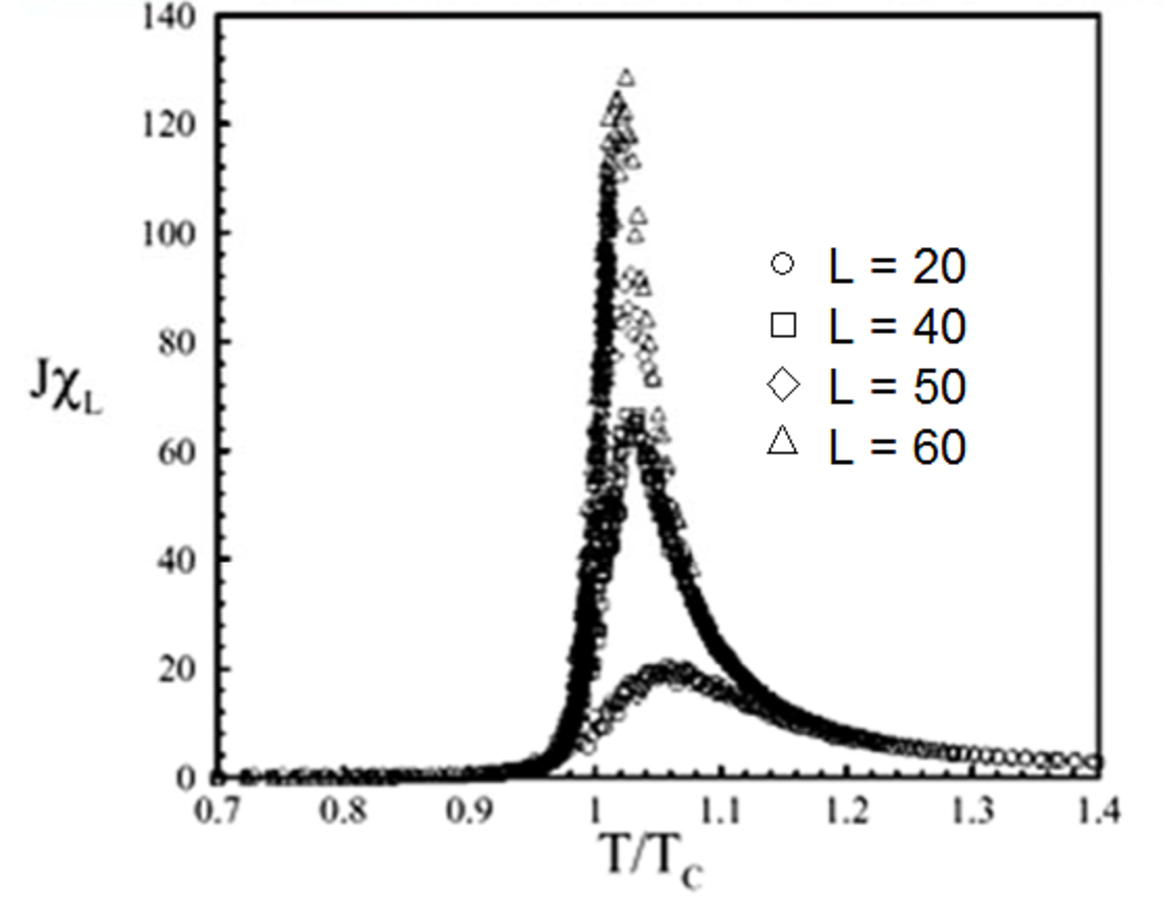
\includegraphics[width=0.9\textwidth]{pics/susce2.pdf}
  \captionof{figure}{Divergence of the magnetic susceptibility for different system sizes. Note that the divergence is more pronounced for larger system sizes.}
  \label{fig:susce2.pdf}
\end{minipage}
\end{minipage}
\vspace{0.1cm}

\subsection{Binder Cumulant}

Binder defined a quantity, which is meant to be independent of the system size L at $T_c$:
\begin{equation}
U_L\equiv 1-\frac{\avkl{M^4}_L}{3\avkl{M^2}^2_L}
\label{eq:bin_cum}
\end{equation}
This can be easily seen:
$$
\frac{\avkl{M^4}_L}{3\avkl{M^2}^2_L} = \frac{L^\frac{4\beta}{\nu} F_{M4}\ekl{\kl{T-T_c}L^\frac{1}{\nu}}}{\kl{L^\frac{2\beta}{\nu} F_{M2}\ekl{\kl{T-T_c}L^\frac{1}{\nu}}}^2} = F_C\ekl{\kl{T-T_c}L^\frac{1}{\nu}}
$$
If $T=T_C$, then the scaling function $F_C$, which is just the ratio of two other scaling functions, is a constant which is independent of the lattice size. For $T>T_C$, the magnetization follows a Gaussian distribution according to 
$$P_L\kl{M}=\sqrt{\frac{L^d}{\pi\sigma_L}}\text{exp}\ekl{-\frac{M^2L^d}{\sigma_L}},
$$ 
with $\sigma_L=k_BT2\chi_L$. Since the fourth moment equals three times the second  moment squared $\kl{\avkl{M^4}=3\avkl{M^2}^2_L}$ it follows that $U_L$ must be zero. Below the critical temperature ($T<T_c$) there are two ground states in the ordered phase (one with positive and one with negative magnetization).
\begin{equation}
P_L\kl{M}=\frac{1}{2}\sqrt{\frac{L^d}{\pi\sigma_l}}\mkl{\text{exp}\ekl{-\frac{\kl{M-M_S}^2L^d}{\sigma_L}}+\text{exp}\ekl{-\frac{\kl{M+M_S}^2L^d}{\sigma_L}}}
\label{eq:dbl_grnd_state}
\end{equation}
For this distribution, it holds that $\avkl{M^4}=\avkl{M^2}^2_L$ and therefore $U_L=\frac{2}{3}$. This means that 
\begin{equation}
U_L =\begin{cases}
  \frac{2}{3} & \text{for }T<T_c\\
  \text{const.} & \text{for }T=T_c\\
 0 & \text{for }T>T_c
\end{cases}
\end{equation}

\vspace{0.1cm}
\noindent
\begin{minipage}{\textwidth}
\begin{minipage}{\textwidth}
This is the most efficient way to calculate the critical temperature, since the Binder cumulant $U_L$ is a quantity which is very sensitive to the temperature. For infinite systems it shows a jump at $T_c$.
\end{minipage}
\begin{minipage}{\textwidth}
  \centering
  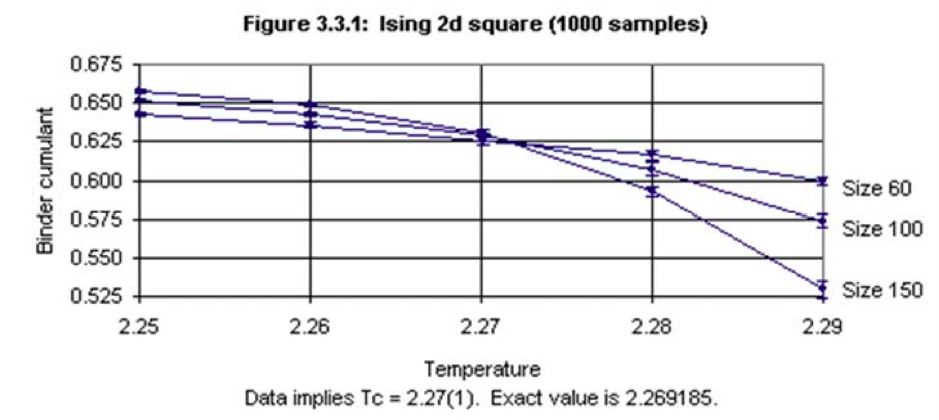
\includegraphics[height=200pt]{pics/bin_cum}
  \captionof{figure}{Binder cumulant for 2D finite systems in the Ising model.}
  \label{fig:bin_cum}
\end{minipage}
\end{minipage}
\vspace{0.1cm}


\vspace{0.1cm}
\noindent
\begin{minipage}{\textwidth}
\begin{minipage}{\textwidth}
The divergence of quantities such as the magnetization, is only approximated as a simple power law. Far away from $T_c$ they do not follow this ansatz anymore, and corrections have to be made. We can observe the subdominant effects of this by calculating the Binder cumulants for small system sizes.
\end{minipage}
\begin{minipage}{\textwidth}
  \centering
  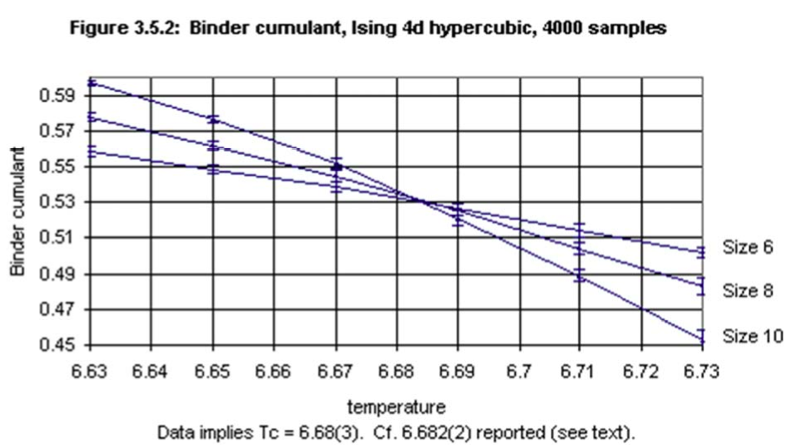
\includegraphics[height=200pt]{pics/bin_cum_4D}
  \captionof{figure}{4D finite systems for the Ising model. Note that the lines do not cross all at the same point.}
  \label{fig:bin_cum2}
\end{minipage}
\end{minipage}
\vspace{0.1cm}

$$M\kl{T} = A_0\kl{T_c-T}^{\beta_0} + A_1\kl{T_c-T}^{\beta_1} + ... $$
$$\xi\kl{T} = C_0\kl{T_c-T}^{\nu_0} + C_1\kl{T_c-T}^{\nu_1} + ... $$
with $\beta_1>\beta$ and $\nu_1<\nu$. These corrections are very important for high quality data, where the errors are small and the deviations become visible. The scaling functions must also be generalized as
$$M\kl{T,L}=
L^{\frac{\beta}{\nu}} F_{M} \ekl{\kl{T-T_c}L^{\frac{1}{\nu}}} +
L^{x} F^1_{M} \ekl{\kl{T-T_c}L^{\frac{1}{\nu}}}+...
$$
with $x=max\ekl{\frac{\beta}{\nu},\frac{\beta}{\nu_1},\frac{\beta}{\nu}-1}$.

\subsection{First Order Transition}
\label{subsec:first_order_trans}

Until now, we only considered critical points for a second order transition, which is characterized by a discontinuity in the second derivative of the free energy (e.g., at the critical temperature). There are also other kinds of transitions, which are characterized by their \emph{order} by means of the $n^{th}$ derivative of the free energy not being continuous. We call those transitions, for which the lowest non-continuous derivative is of order n, $n^{th}$ \emph{order phase transitions}. For $T<T_c$, the Ising model has a jump in the magnetization at $H=0$   (from minus to plus, by varying the field H), which is proportional the first derivative of the free energy. This leads to the susceptibility assuming a delta peak at $H=0$. This kind of phase transition is more common in nature than second order transitions.



\begin{figure}[h!]
		\centering
        \begin{subfigure}[]{0.45\textwidth}
                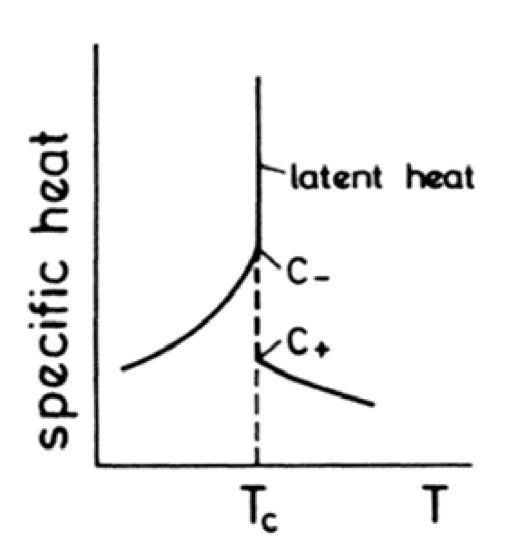
\includegraphics[height=0.9\textwidth]{pics/first_order_heat}
                \caption{Specific heat}
                \label{fig:first_order_heat}
        \end{subfigure}%
~
       \begin{subfigure}[]{0.45\textwidth}
                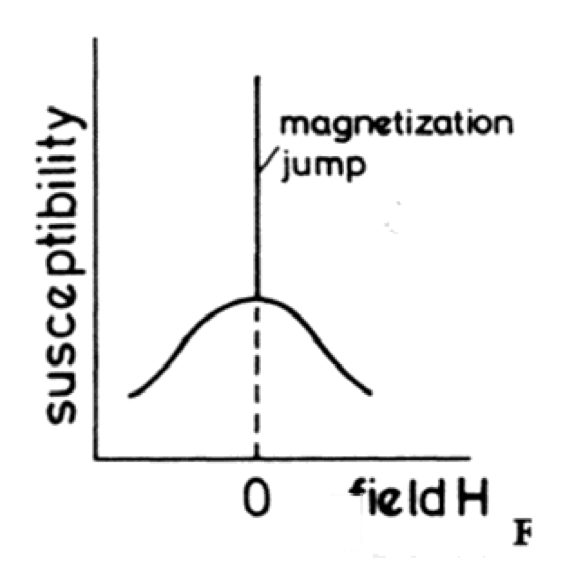
\includegraphics[height=0.85\textwidth]{pics/first_order_magnetization}
                \caption{Susceptibility}
                \label{fig:first_order_magnetization}
        \end{subfigure}
        \caption{First order transitions}
	\label{fig:animals}
\end{figure}


\begin{comment}
\vspace{0.1cm}
\noindent
\begin{minipage}{\textwidth}
\begin{minipage}{.48\textwidth}
  \centering
  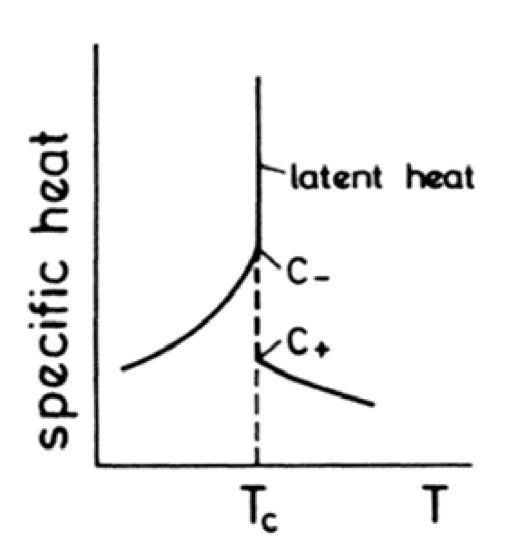
\includegraphics[width=0.9\textwidth]{pics/first_order_heat}
  \captionof{figure}{First order transition manifested in the specific heat.}
  \label{fig:first_order_heat}
\end{minipage}\hfill
\begin{minipage}{.48\textwidth}
  \centering
  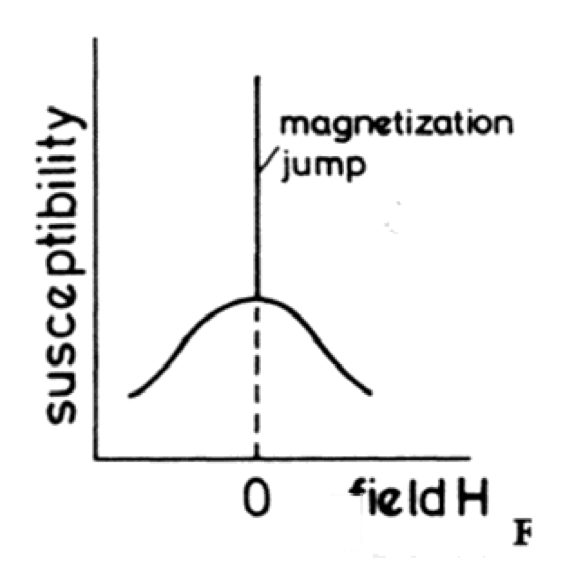
\includegraphics[width=0.9\textwidth]{pics/first_order_magnetization}
  \captionof{figure}{First order transition manifested in the susceptibility.}
  \label{fig:first_order_magnetization}
\end{minipage}
\end{minipage}
\vspace{0.1cm}
%\end{comment}

\noindent
\begin{minipage}{\textwidth}
\begin{minipage}{.38\textwidth}
Usual symptoms of a first order transition are magnetization jumps in small systems (See Fig \ref{fig:magn_jump}), or the hysteresis. In infinite lattices this is not possible since the jump to a ground state of opposite sign would take an infinite (Monte Carlo) time to happen. 
\end{minipage}\hfill
\begin{minipage}{.6\textwidth}
\centering
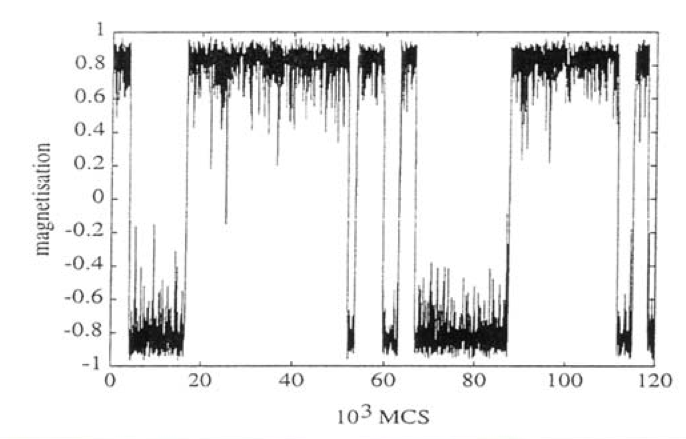
\includegraphics[width=0.95\textwidth]{pics/magn_jump}
\captionof{figure}{First order transitions.}
\label{fig:magn_jump}
\end{minipage}
\end{minipage}

\vspace{0.1cm}

Binder derived that if the distribution of the magnetization is described by two Gaussians, the magnetization (in dependence on the field $H$) has the form of a $\text{tanh}(\alpha L^d)$. Consequently, susceptibility can be calculated by differentiating the magnetization with respect to the field $H$:
\begin{align}
M(H) &= \chi_L^D H + M_L \text{tanh}\kl{\beta H M_L L^d}\\
\chi_L\kl{H} &= \pder{M}{H} = \chi_L^D + \frac{\beta M_L L^d}{\text{cosh}^2\kl{\beta H M_L L^d}}.
\end{align}
Similarly to the scaling for the second order transition, we can scale the maximum of the susceptibility ($\chi_L\kl{H=0}\propto L^d$) and the width of the peak ($\Delta\chi_L\propto L^{-d}$).


\vspace{0.1cm}
\noindent\begin{minipage}{\textwidth}
\begin{minipage}{0.48\textwidth}
  \centering
  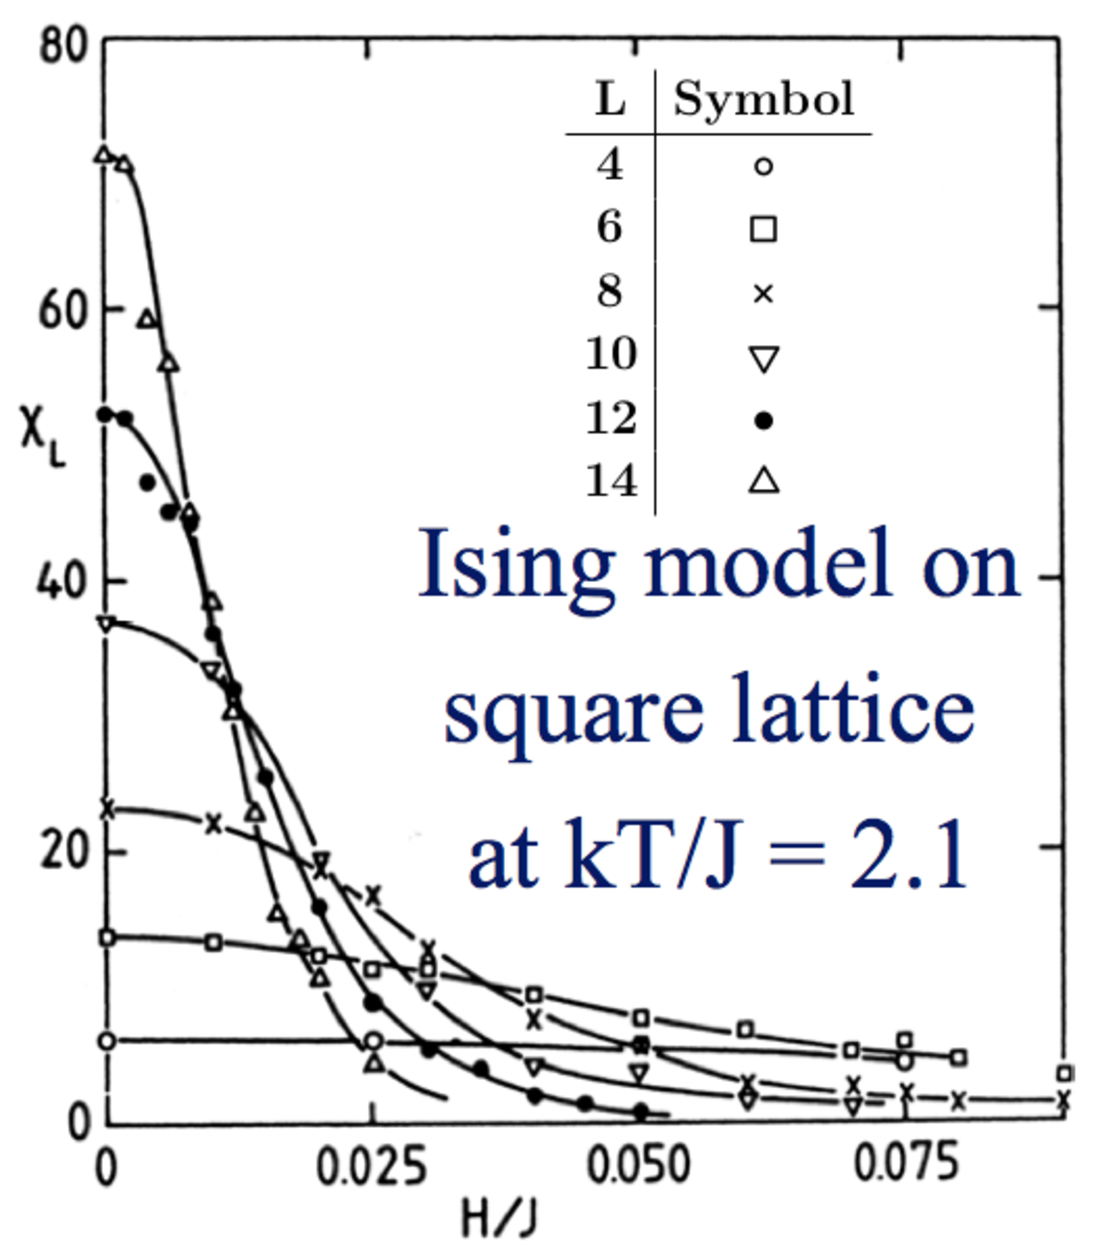
\includegraphics[width=.95\textwidth]{pics/unscaled_susce.pdf}
  \captionof{figure}{Susceptibility for different system sizes in the Ising model.}
  \label{fig:unscaled_susce}
\end{minipage}\hfill
\begin{minipage}{.48\textwidth}
  \centering
  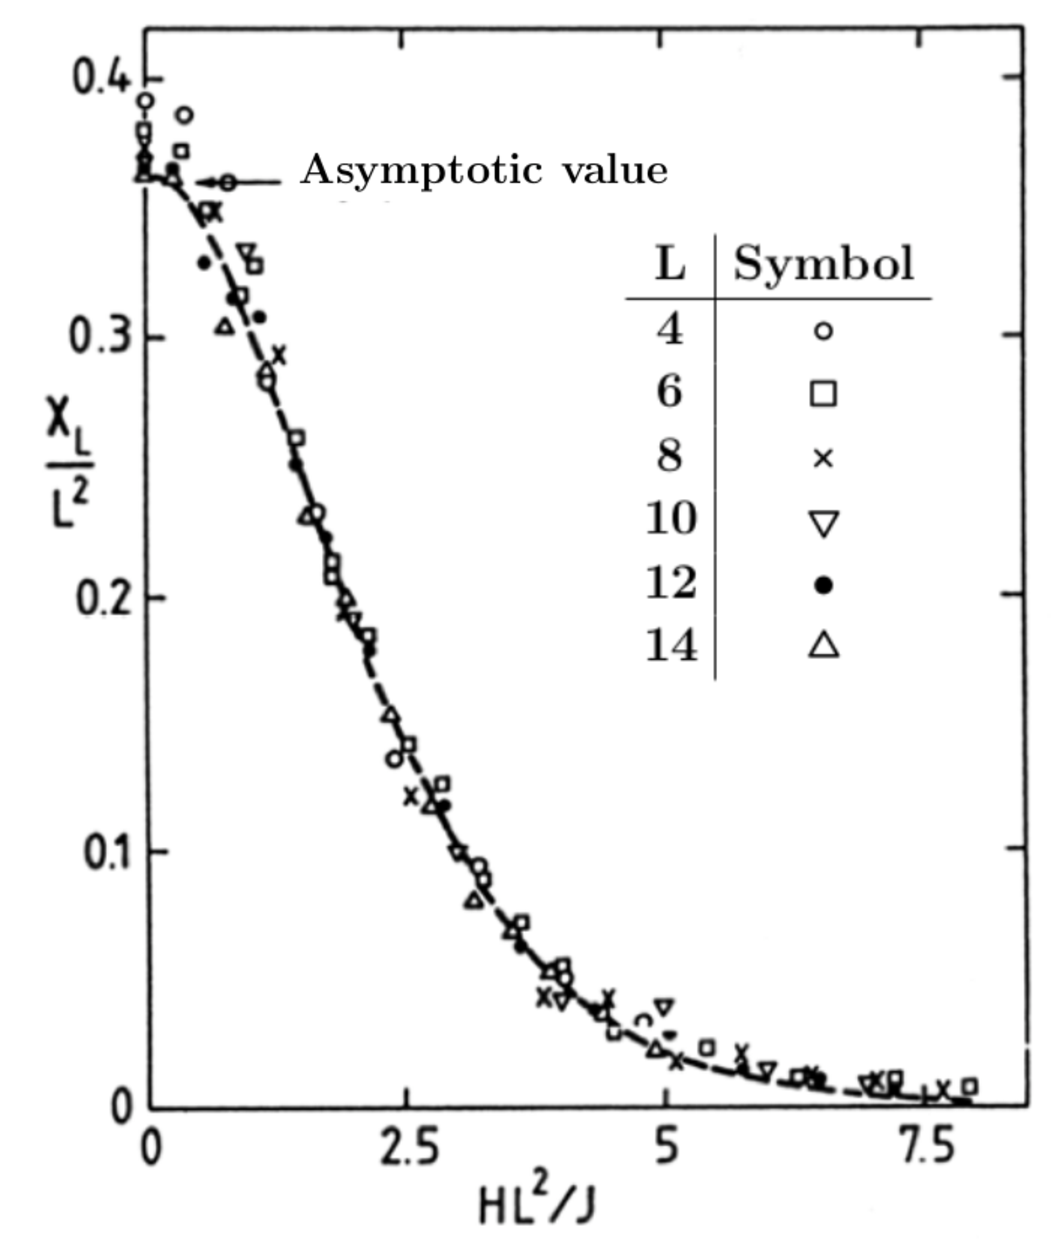
\includegraphics[width=.95\textwidth]{pics/scaled_susce.pdf}
  \captionof{figure}{Data Collapse for scaled susceptibility for different system sizes in the Ising model.}
  \label{fig:scaled_susce}
\end{minipage}
\end{minipage}
\vspace{0.1cm}



